\section*{Resolução da Questão 4: Verificação de Consistências em CSP}

\subsection*{A) Declaração Formal do Problema}

O paradigma CSP (Constraint Satisfaction Problem) exige o delineamento exato da alocação da equipe médica:

\begin{itemize}
    \item \textbf{Conjunto Alvo ($V$):} As vagas que demandam escala: $V = \{T_1, T_2, T_3, T_4, T_5, T_6\}$.
    \item \textbf{Opções Universais ($D$):} A bateria de profissionais autorizados para o cargo em cada vaga: $D_i = \{A, B, C, D\}$.
    \item \textbf{Regras Unitárias (1 nó):} Bloqueio pessoal. $T_3 \neq A$ (Médico A de folga no 3º).
    \item \textbf{Regras Binárias (2 nós):} 
    \begin{itemize}
        \item Vedação de turnos empilhados: $T_i \neq T_{i+1}$.
        \item Impedimento cruzado C-C: $\neg(T_2 = C \land T_5 = C)$.
    \end{itemize}
    \item \textbf{Regras Multi-nós (Globais):}
    \begin{itemize}
        \item Obrigatoriedade B: $B \in \{T_1, T_2\}$.
        \item Teto de Carga Horária D: Ocorrências $(T_i = D) \leq 2$.
    \end{itemize}
\end{itemize}

\textbf{Rede de Restrições Estruturais:}

\begin{center}
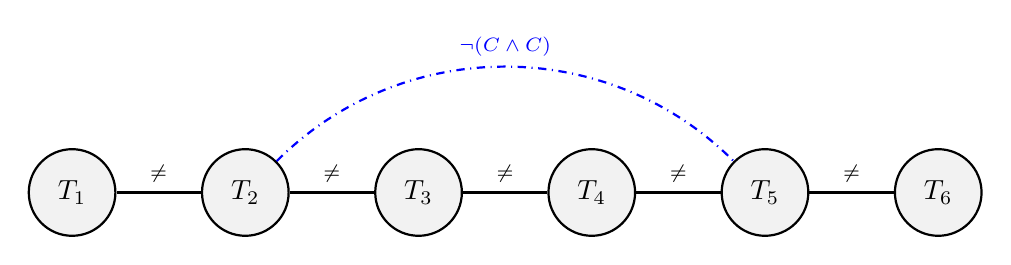
\begin{tikzpicture}[
    node distance=2.2cm,
    var/.style={circle, draw=black, thick, fill=gray!10, minimum size=1.1cm},
    edge/.style={-, thick}
]
    \node[var] (T1) {$T_1$};
    \node[var, right of=T1] (T2) {$T_2$};
    \node[var, right of=T2] (T3) {$T_3$};
    \node[var, right of=T3] (T4) {$T_4$};
    \node[var, right of=T4] (T5) {$T_5$};
    \node[var, right of=T5] (T6) {$T_6$};

    \draw[edge] (T1) -- (T2) node[midway, above] {\scriptsize $\neq$};
    \draw[edge] (T2) -- (T3) node[midway, above] {\scriptsize $\neq$};
    \draw[edge] (T3) -- (T4) node[midway, above] {\scriptsize $\neq$};
    \draw[edge] (T4) -- (T5) node[midway, above] {\scriptsize $\neq$};
    \draw[edge] (T5) -- (T6) node[midway, above] {\scriptsize $\neq$};
    
    \draw[dashdotted, blue, thick, bend left=45] (T2) to node[midway, above] {\scriptsize $\neg(C \land C)$} (T5);
\end{tikzpicture}
\end{center}

\subsection*{B) Rastreio de Backtracking Puro}

Rodando o DFS sem inteligência prévia, pela via lexicográfica cega:

\begin{table}[H]
\centering
\begin{tabular}{|c|c|l|}
\hline
\textbf{Step} & \textbf{Injeção} & \textbf{Diagnóstico da Consistência} \\ \hline
1 & $T_1 = A$ & Aceito \\ \hline
2 & $T_2 = A$ & Quebra de regra de empilhamento \\ \hline
3 & $T_2 = B$ & Aceito \\ \hline
4 & $T_3 = A$ & Quebra da folga do Médico A \\ \hline
5 & $T_3 = B$ & Quebra de regra de empilhamento \\ \hline
6 & $T_3 = C$ & Aceito \\ \hline
7 & $T_4 = A$ & Aceito \\ \hline
8 & $T_5 = A$ & Quebra de regra de empilhamento \\ \hline
9 & $T_5 = B$ & Aceito \\ \hline
10 & $T_6 = A$ & Consolidado com Êxito Total \\ \hline
\end{tabular}
\end{table}

Apenas pela sorte da ordenação inicial, 0 saltos reversos estruturais (backtracks pesados onde um nó inteiro falha) foram necessários. A montagem esbarrou em 4 becos rápidos e seguiu.

\subsection*{C) Aceleração Heurística (MRV e Degree)}

\begin{itemize}
    \item \textbf{Tática do Domínio Mínimo (MRV):} Vasculha quem tem o cinto de restrições mais apertado. $T_3$ possuía domínio nativo de apenas 3 profissionais devido à folga de A. Escolhê-lo primeiro corta raízes falhas gigantescas do espaço global.
    \item \textbf{Tática do Grau de Conexão (Degree):} Como desempate, pega-se o hub com mais cordas conectadas (ex: $T_2$, amarrado a $T_1, T_3, T_5$). Fixar $T_2$ estrangula fortemente o oxigênio (domínio) de todo o sistema simultaneamente, forçando fracassos e podas vitais cedo na árvore de busca.
\end{itemize}

\subsection*{D) Antecipação Lógica (Forward Checking)}

Ao fechar um nó, retiram-se as opções proibidas do radar dos nós futuros:

\begin{table}[H]
\centering
\resizebox{\textwidth}{!}{
\begin{tabular}{|l|l|}
\hline
\textbf{Commit} & \textbf{Sobras Lógicas nas Caixas Futuras} \\ \hline
$T_1 = A$ & $T_2: \{B\}$, $T_3: \{B, C, D\}$, Inalterados: $T_{4..6}$ \\ \hline
$T_2 = B$ & $T_3: \{C, D\}$, $T_4: \{A, B, C, D\}$, Inalterados: $T_{5..6}$ \\ \hline
$T_3 = C$ & $T_4: \{A, B, D\}$, Inalterados: $T_{5..6}$ \\ \hline
$T_4 = A$ & $T_5: \{B, C, D\}$, Inalterados: $T_6$ \\ \hline
$T_5 = B$ & $T_6: \{A, C, D\}$ \\ \hline
$T_6 = A$ & Escala Fechada. \\ \hline
\end{tabular}
}
\end{table}

A checagem reduziu o trajeto inteiro de 10 injeções (do Backtracking) para míseras \textbf{6 atuações perfeitas}. Todo movimento proibido havia sido apagado da tabela por clarividência sistêmica.

\subsection*{E) Saltos Otimizados via Backjumping (CBJ)}

O mecanismo de salto dirigido por conflito ignora o retorno cronológico tradicional, agindo de forma radical.

\begin{itemize}
    \item \textbf{Gestão da Culpa:} Toda variável rastreia intimamente quais vizinhos do passado amputaram seu domínio. Se o balde de um $T_5$ zerasse, ele não devolveria a bola para $T_4$ no cego. Ele verificaria seu \textit{Conflict Set} e acusaria pontualmente $T_2$, ordenando o retrocesso espacial direto para ele.
    \item \textbf{Impactos no Algoritmo Escalar:} Esta tática extirpa integralmente a exploração de galhos mortos (thrashing), pois varre as causas subjacentes dos problemas em vez de insistir em variáveis irrelevantes adjacentes que nada poderiam fazer para resgatar a consistência.
\end{itemize}
